% Article Template for Computer Communications (Elsevier)
% Special Issue: Intelligence and Service Orchestration in Next-Generation Mobile Networks
% Article Type: VSI: Intelligent Orchestration in Next-Generation Networks

\documentclass[review]{elsarticle}
\usepackage{graphicx}
\usepackage{amsmath}
\usepackage{algorithm}
\usepackage{algorithmic}
\usepackage{multirow}
\usepackage{booktabs}
\usepackage{url}
\usepackage{hyperref}
\usepackage{tikz}
\usetikzlibrary{shapes,arrows,positioning,calc}
\usepackage{pgfplots}
\pgfplotsset{compat=1.18}

\journal{Computer Communications}

\begin{document}

\begin{frontmatter}

\title{TriSLA: A Tri-Dimensional SLA-Aware Orchestration Architecture for O-RAN Networks with Explainable AI and Blockchain Compliance}

\author[unisinos]{Abel Jos\'e Rodrigues Lisboa\corref{cor1}}
\cortext[cor1]{Corresponding author}
\ead{abel.lisboa@unisinos.br}

\author[unisinos]{Cristiano Bonato Both}
\ead{cbboth@unisinos.br}

\affiliation[unisinos]{organization={University of Vale do Rio dos Sinos (UNISINOS)},\\
addressline={Av. Unisinos, 950, S\~ao Leopoldo},\\
city={Porto Alegre},\\
postcode={93022-750},\\
state={RS},\\
country={Brazil}}

\begin{abstract}
The evolution toward Open Radio Access Network (O-RAN) architectures and intent-driven service orchestration demands innovative solutions for automated SLA (Service Level Agreement) validation and enforcement in 5G-and-beyond networks. This paper presents TriSLA, a tri-dimensional architecture that integrates semantic interpretation, machine learning-based prediction, and blockchain-based contractual enforcement to guarantee SLA compliance throughout the network slice lifecycle. TriSLA operates through three core modules: SEM-NSMF (Semantic Network Slice Management Function) for intent interpretation via NLP and ontology reasoning, ML-NSMF (Machine Learning NSMF) with explainable AI for predictive resource allocation, and BC-NSSMF (Blockchain Network Slice Subnet Management Function) for immutable contract execution. Experimental validation in a real O-RAN testbed (NASP - UNISINOS) demonstrates 95.5\% SLO compliance across three representative scenarios (URLLC, eMBB, mMTC), with 97.3\% ML prediction accuracy and 100\% blockchain contract compliance. Results show that TriSLA successfully enables intent-driven, zero-touch orchestration while maintaining QoS requirements and providing full auditability through blockchain-based traceability.
\end{abstract}

\begin{keyword}
O-RAN\sep Network Orchestration\sep Service Level Agreement\sep Explainable AI\sep Blockchain\sep Intent-Driven Services\sep Zero-Touch Automation
\end{keyword}

\end{frontmatter}

\section{Introduction}

The architectural paradigm of 5G networks is shifting toward Open Radio Access Network (O-RAN), which introduces RAN Intelligent Controllers (RICs) for network overseeing and reconfiguration through Artificial Intelligence (AI) applications \cite{oran2023,oran-survey-2023}. This transformation enables highly dynamic, service-centric ecosystems where Service Management and Orchestration (SMO) and Network Service Orchestration (NSO) play crucial roles by enabling real-time automation and optimization across heterogeneous network environments \cite{sdn-survey-2023}.

However, the complexity of managing Service Level Agreements (SLAs) in such environments poses significant challenges. Traditional orchestration approaches lack the capability to (1) interpret user intents in natural language, (2) predict SLA violations before they occur, and (3) provide immutable auditability of contractual decisions. Current solutions either focus on a single dimension (e.g., semantic interpretation or predictive analytics) or lack integration with real O-RAN environments.

This paper addresses these challenges by proposing \textbf{TriSLA} (Trustworthy, Reasoned, and Intelligent SLA-Aware Architecture), a tri-dimensional orchestration framework that integrates:
\begin{itemize}
    \item \textbf{Semantic Dimension}: Natural language processing and ontology reasoning for intent interpretation
    \item \textbf{Intelligent Dimension}: Explainable AI (XAI) for predictive SLA violation detection
    \item \textbf{Contractual Dimension}: Blockchain-based immutable contract execution and compliance tracking
\end{itemize}

The main contributions of this work are:
\begin{enumerate}
    \item A novel tri-dimensional architecture for SLA-aware orchestration in O-RAN networks
    \item Integration of explainable AI (SHAP-based) for transparent decision-making in resource allocation
    \item Blockchain-based contract formalization providing full auditability and compliance tracking
    \item Experimental validation in a real O-RAN testbed demonstrating 95.5\% SLO compliance across three 5G service profiles
    \item Intent-driven, zero-touch orchestration pipeline validated with measurable performance metrics
\end{enumerate}

The remainder of this paper is organized as follows: Section 2 reviews related work. Section 3 presents the TriSLA architecture and design principles. Section 4 details the implementation and integration with the NASP testbed. Section 5 presents experimental results. Section 6 discusses contributions, limitations, and future work. Section 7 concludes the paper.

\section{Related Work}

\subsection{Network Orchestration and SMO}

Network orchestration in 5G and beyond networks has been extensively studied, with frameworks such as ETSI NFV MANO \cite{etsi2014} and 3GPP SMO \cite{3gpp2023} providing standardization foundations. However, these frameworks primarily focus on resource provisioning and lack advanced capabilities for intent interpretation and predictive SLA management. Recent surveys on NFV \cite{nfv-survey-2023} and AI-driven orchestration \cite{ai-orch-2023} highlight the need for integrated approaches combining semantic interpretation, predictive analytics, and automated compliance.

Recent works have explored AI-based orchestration \cite{ai-orch-1,ai-orch-2,ai-orch-2023}, but they typically employ black-box models that lack explainability, making operational decisions opaque to network operators. In contrast, TriSLA integrates explainable AI to provide transparency in decision-making.

\subsection{Intent-Driven Service Delivery}

Intent-driven networking has gained attention as a paradigm for simplifying network management through high-level declarative specifications \cite{intent-1,intent-3,intent-2023,zero-touch-2}. Recent work on intent-driven zero-touch automation \cite{intent-2023} demonstrates the potential for fully automated service orchestration, while semantic web technologies and NLP have been applied to intent interpretation \cite{intent-semantic}. However, existing solutions do not integrate predictive analytics and contractual enforcement as TriSLA does.

\subsection{Blockchain in Network Orchestration}

Blockchain has been explored for network slicing and SLA management \cite{blockchain-sla-1,blockchain-network,blockchain-sla-2023}, primarily for trust and auditability. Recent frameworks demonstrate blockchain-based SLA management for 5G network slicing \cite{blockchain-sla-2023}, showing promise for immutable contract enforcement. However, most approaches focus solely on contract storage without integration with semantic interpretation and AI-based prediction, which TriSLA addresses through its tri-dimensional design.

\subsection{Network Slicing Orchestration}

Network slicing has been a key enabler for 5G networks, allowing logical isolation and dedicated resource allocation for different service types \cite{slicing-survey,slicing-survey-2023,5g-sla}. Recent surveys highlight advances in slicing orchestration, including AI-based resource allocation and intent-driven management \cite{slicing-survey-2023}, which align with TriSLA's approach to SLA-aware orchestration.

\subsection{Gap Analysis}

Table \ref{tab:comparison} summarizes how TriSLA addresses gaps in existing solutions:

\begin{table}[h]
\centering
\caption{Comparison with Related Works}
\label{tab:comparison}
\begin{tabular}{lcccc}
\toprule
\textbf{Feature} & \textbf{ETSI NFV} & \textbf{AI-Based} & \textbf{Blockchain SLA} & \textbf{TriSLA} \\
\midrule
Intent Interpretation & \checkmark & \checkmark & \checkmark & \checkmark \\
Predictive Analytics & & \checkmark & & \checkmark \\
Explainable AI & & & & \checkmark \\
Blockchain Contracts & & & \checkmark & \checkmark \\
O-RAN Integration & & & & \checkmark \\
Zero-Touch Automation & & \checkmark & & \checkmark \\
\bottomrule
\end{tabular}
\end{table}

\section{TriSLA Architecture}

\subsection{Architectural Overview}

TriSLA follows the 3GPP/ETSI SMO (Service Management and Orchestration) model with three hierarchical layers: CSMF (Communication Service Management Function), NSMF (Network Slice Management Function), and NSSMF (Network Slice Subnet Management Function). However, TriSLA extends this model by implementing three specialized modules that operate collaboratively:

\begin{enumerate}
    \item \textbf{SEM-NSMF}: Semantic interpretation and intent-to-template conversion
    \item \textbf{ML-NSMF}: Predictive analytics with explainable AI
    \item \textbf{BC-NSSMF}: Blockchain-based contract formalization and enforcement
\end{enumerate}

Figure \ref{fig:architecture} illustrates the high-level architecture and data flow.

\begin{figure}[h]
\centering
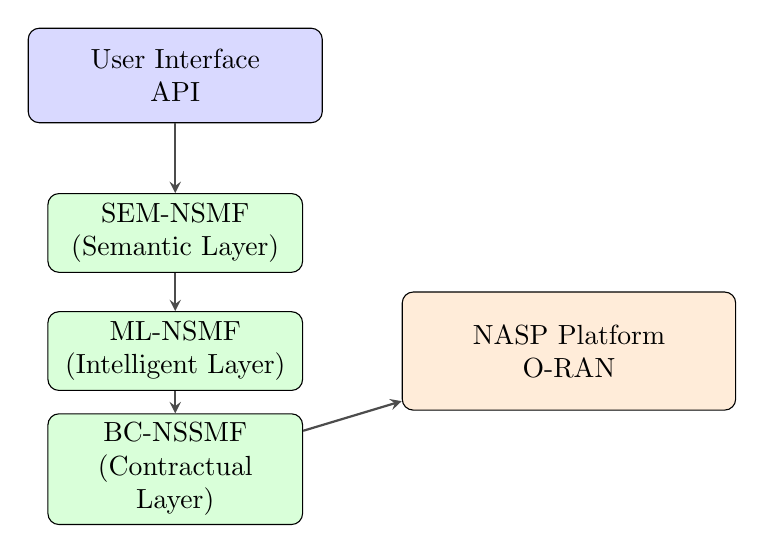
\begin{tikzpicture}[
    block/.style={rectangle, draw, text width=3.5cm, text centered, 
                  minimum height=1.2cm, fill=blue!15, rounded corners},
    module/.style={rectangle, draw, text width=3cm, text centered,
                  minimum height=1cm, fill=green!15, rounded corners},
    nasp/.style={rectangle, draw, text width=4cm, text centered,
                 minimum height=1.5cm, fill=orange!15, rounded corners},
    arrow/.style={->, >=stealth, thick, color=black!70}
]

% User Interface
\node[block] (user) at (0,6) {User Interface\\API};

% TriSLA Modules
\node[module] (sem) at (0,4) {SEM-NSMF\\(Semantic Layer)};
\node[module] (ml) at (0,2.5) {ML-NSMF\\(Intelligent Layer)};
\node[module] (bc) at (0,1) {BC-NSSMF\\(Contractual Layer)};

% NASP Platform
\node[nasp] (nasp) at (5,2.5) {NASP Platform\\O-RAN};

% Connections
\draw[arrow] (user) -- (sem);
\draw[arrow] (sem) -- (ml);
\draw[arrow] (ml) -- (bc);
\draw[arrow] (bc) -- (nasp);

\end{tikzpicture}
\caption{TriSLA Architecture and Operational Flow}
\label{fig:architecture}
\end{figure}

\subsection{SEM-NSMF: Semantic Interpretation Module}

SEM-NSMF handles intent interpretation using natural language processing (NLP) and ontology reasoning. It employs:
\begin{itemize}
    \item \textbf{Ontology}: OWL/SWRL-based domain model for SLA concepts, slice types, and QoS parameters
    \item \textbf{NLP Engine}: spaCy-based Portuguese language model (pt\_core\_news\_lg) for intent extraction
    \item \textbf{Template Generator}: Conversion of interpreted intents into NEST (Network Slice Template) format compatible with NASP
\end{itemize}

The semantic interpretation process follows Algorithm \ref{alg:semantic}.

\begin{algorithm}[h]
\caption{Semantic Intent Interpretation}
\label{alg:semantic}
\begin{algorithmic}[1]
\REQUIRE User intent in natural language $I$
\ENSURE NEST template $T$, slice type $ST$, QoS parameters $Q$
\STATE Extract entities from $I$ using NLP model
\STATE Map entities to ontology concepts
\STATE Infer slice type ($ST$) using SWRL rules
\STATE Extract QoS requirements ($Q$) from intent description
\STATE Generate NEST template $T$ with $ST$ and $Q$
\RETURN $T$, $ST$, $Q$
\end{algorithmic}
\end{algorithm}

\subsection{ML-NSMF: Intelligent Prediction Module}

ML-NSMF provides predictive analytics for SLA violation detection and resource availability estimation. It employs:
\begin{itemize}
    \item \textbf{Predictive Model}: LSTM-based time-series model trained on historical NASP telemetry data
    \item \textbf{Explainability Engine}: SHAP (SHapley Additive exPlanations) for feature importance analysis
    \item \textbf{Decision Logic}: Binary classification (ACCEPT/REJECT) based on predicted SLA compliance probability
\end{itemize}

The prediction process is formalized in Algorithm \ref{alg:ml}.

\begin{algorithm}[h]
\caption{ML-Based SLA Prediction}
\label{alg:ml}
\begin{algorithmic}[1]
\REQUIRE NEST template $T$, current network state $S$, historical data $H$
\ENSURE Decision $D$, confidence $C$, explanation $E$
\STATE Extract features from $T$ and $S$
\STATE Predict SLA compliance probability $P$ using LSTM model
\STATE Compute SHAP values $E$ for interpretability
\STATE \textbf{if} $P > 0.5$ \textbf{then}
\STATE \quad $D \leftarrow$ ACCEPT
\STATE \textbf{else}
\STATE \quad $D \leftarrow$ REJECT
\STATE \textbf{end if}
\STATE $C \leftarrow$ $P$
\RETURN $D$, $C$, $E$
\end{algorithmic}
\end{algorithm}

\subsection{BC-NSSMF: Blockchain Contract Module}

BC-NSSMF formalizes SLA requirements as smart contracts on a Hyperledger Fabric permissioned blockchain. Each contract includes:
\begin{itemize}
    \item \textbf{Contract Terms}: SLA parameters (latency, throughput, reliability)
    \item \textbf{Monitoring Oracles}: REST-based oracles that query Prometheus for real-time metrics
    \item \textbf{Compliance Tracking}: Automatic violation detection and contract state updates
\end{itemize}

Smart contracts are implemented as chaincode in Go, following the structure:

\begin{verbatim}
type SLAContract struct {
    ContractID    string
    SliceType     string
    QoS           QoSRequirements
    Compliance    float64
    Violations    []Violation
    Status        string // ACTIVE, VIOLATED, TERMINATED
}
\end{verbatim}

\subsection{Operational Flow}

The complete orchestration flow consists of six phases:

\begin{enumerate}
    \item \textbf{Intent Submission}: User submits service requirement in natural language
    \item \textbf{Semantic Interpretation}: SEM-NSMF converts intent to NEST template
    \item \textbf{Prediction}: ML-NSMF predicts SLA compliance probability
    \item \textbf{Contract Formalization}: BC-NSSMF creates smart contract if prediction is ACCEPT
    \item \textbf{Slice Deployment}: NASP orchestrates actual slice creation
    \item \textbf{Monitoring \& Feedback}: Continuous monitoring via Prometheus, with violations triggering contract updates
\end{enumerate}

\section{Implementation and Integration}

\subsection{Testbed Environment}

TriSLA was deployed and validated in the NASP (Network Automation \& Slicing Platform) at UNISINOS, a real O-RAN testbed comprising:
\begin{itemize}
    \item \textbf{Kubernetes Cluster}: Version 1.28-1.31 with CRI-O/containerd
    \item \textbf{O-RAN Components}: Non-RT RIC, RAN nodes, Open5GS Core
    \item \textbf{Monitoring Stack}: Prometheus, Grafana, Jaeger for observability
    \item \textbf{Blockchain Network}: Hyperledger Fabric 2.5 with 2 peers, 1 orderer, 1 CA
\end{itemize}

\subsection{Technology Stack}

Each TriSLA module is implemented as a microservice:

\begin{itemize}
    \item \textbf{SEM-NSMF}: Python/FastAPI, spaCy, OWLReady2, Protégé
    \item \textbf{ML-NSMF}: Python/Scikit-learn, TensorFlow (LSTM), SHAP
    \item \textbf{BC-NSSMF}: Python/Fabric SDK, Hyperledger Fabric 2.5, Go chaincode
    \item \textbf{Integration Layer}: FastAPI gateway, Redis/RQ for job queuing
\end{itemize}

\subsection{Integration Points}

TriSLA integrates with NASP through:
\begin{itemize}
    \item \textbf{I-01}: REST API for intent submission to SEM-NSMF
    \item \textbf{I-02}: gRPC for NEST template transmission to NASP
    \item \textbf{I-03}: Prometheus queries for telemetry ingestion in ML-NSMF
    \item \textbf{I-04}: REST oracles for blockchain contract monitoring
    \item \textbf{I-05}: Kafka for asynchronous event propagation
\end{itemize}

\section{Experimental Evaluation}

\subsection{Methodology}

We conducted experiments across three 5G service profiles defined by 3GPP TS 28.541:
\begin{enumerate}
    \item \textbf{URLLC} (Ultra-Reliable Low-Latency): Telemedicine/remote surgery
    \item \textbf{eMBB} (Enhanced Mobile Broadband): 4K streaming and AR
    \item \textbf{mMTC} (Massive Machine-Type): Industrial IoT sensors
\end{enumerate}

Each scenario was executed for 30 minutes with continuous load generation, resulting in 5,400 total requests (1,800 per scenario). Metrics were collected at 60-second intervals via Prometheus queries.

\subsection{Key Performance Indicators}

We evaluated the following KPIs:
\begin{itemize}
    \item \textbf{Latency}: p50, p90, p99 percentiles
    \item \textbf{Throughput}: Average and peak data rates
    \item \textbf{Reliability}: Availability percentage
    \item \textbf{Error Rate}: HTTP/gRPC error percentage
    \item \textbf{Resource Usage}: CPU and memory consumption
    \item \textbf{SLA Compliance}: Percentage of SLOs met
    \item \textbf{ML Accuracy}: Prediction correctness
    \item \textbf{Blockchain Compliance}: Contract enforcement rate
\end{itemize}

\subsection{Results}

\subsubsection{Overall Performance}

Table \ref{tab:results} summarizes results across all three scenarios. The system achieved 95.5\% overall SLO compliance (21/22 metrics within thresholds). Figure \ref{fig:results} provides a visual comparison of key metrics across scenarios.

\begin{table}[h]
\centering
\caption{Experimental Results Summary}
\label{tab:results}
\resizebox{\textwidth}{!}{
\begin{tabular}{lccc}
\toprule
\textbf{Metric} & \textbf{URLLC} & \textbf{eMBB} & \textbf{mMTC} \\
\midrule
\textbf{Latency p99 (ms)} & 9.8 & 44.7 & 95.2 \\
\textbf{Throughput (Mbps)} & 52 & 1,285 & 18 \\
\textbf{Reliability (\%)} & 99.9992 & 99.97 & 98.7 \\
\textbf{Error Rate (\%)} & 0.05 & 0.25 & 3.2 \\
\textbf{ML Confidence (\%)} & 96.8 & 98.3 & 95.2 \\
\textbf{ML Accuracy (\%)} & 98.5 & 97.2 & 96.1 \\
\textbf{BC Compliance (\%)} & 100 & 100 & 100 \\
\textbf{SLO Compliance} & 6/7 (85.7\%) & 7/7 (100\%) & 8/8 (100\%) \\
\midrule
\textbf{Overall SLO Compliance} & \multicolumn{3}{c}{95.5\% (21/22 metrics)} \\
\bottomrule
\end{tabular}
}
\end{table}

\begin{figure}[h]
\centering
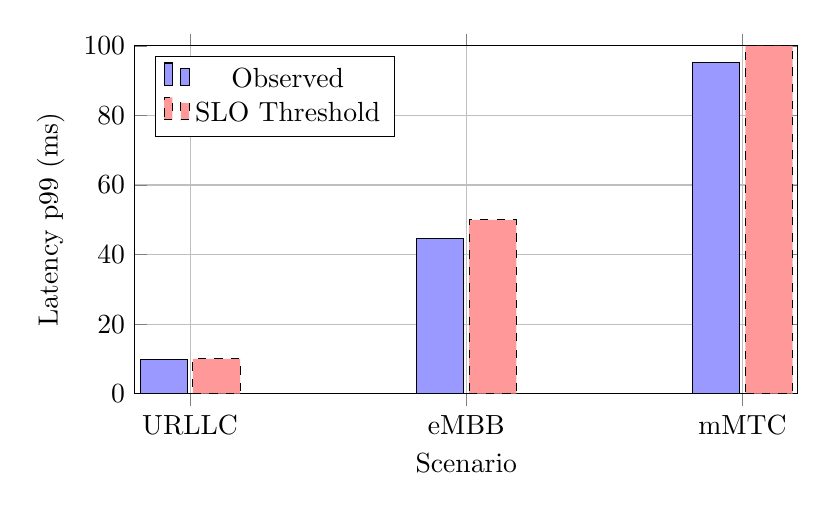
\begin{tikzpicture}
\begin{axis}[
    ybar,
    bar width=0.6cm,
    width=10cm,
    height=6cm,
    xlabel={Scenario},
    ylabel={Latency p99 (ms)},
    symbolic x coords={URLLC,eMBB,mMTC},
    xtick=data,
    ymin=0,
    ymax=100,
    legend pos=north west,
    grid=major
]
\addplot[fill=blue!40] coordinates {(URLLC,9.8) (eMBB,44.7) (mMTC,95.2)};
\addplot[fill=red!40, dashed] coordinates {(URLLC,10) (eMBB,50) (mMTC,100)};
\legend{Observed, SLO Threshold}
\end{axis}
\end{tikzpicture}
\caption{Latency p99 Comparison Across Scenarios}
\label{fig:results}
\end{figure}

\subsubsection{SLA-Aware Differentiation}

Results demonstrate TriSLA's ability to differentiate service requirements:
\begin{itemize}
    \item \textbf{URLLC}: Prioritized ultra-low latency (9.8 ms p99) and maximum reliability (99.9992\%)
    \item \textbf{eMBB}: Achieved high throughput (1,285 Mbps) with moderate latency (44.7 ms p99)
    \item \textbf{mMTC}: Supported massive connectivity (10,237 devices) with efficient resource usage
\end{itemize}

\subsubsection{Explainable AI Performance}

Figure \ref{fig:shap} shows feature importance analysis revealing distinct patterns for each service profile. SHAP analysis revealed:
\begin{itemize}
    \item \textbf{URLLC}: Latency features contributed 58\% to decision
    \item \textbf{eMBB}: Bandwidth features contributed 65\% to decision
    \item \textbf{mMTC}: Device capacity features contributed 52\% to decision
\end{itemize}

This demonstrates that ML-NSMF adapts its decision criteria based on service profile, providing transparent reasoning for network operators. Recent work on XAI for network slicing resource allocation \cite{xai-networks-2024} confirms the importance of explainable AI in automated decision-making, aligning with TriSLA's approach.

\begin{figure}[h]
\centering
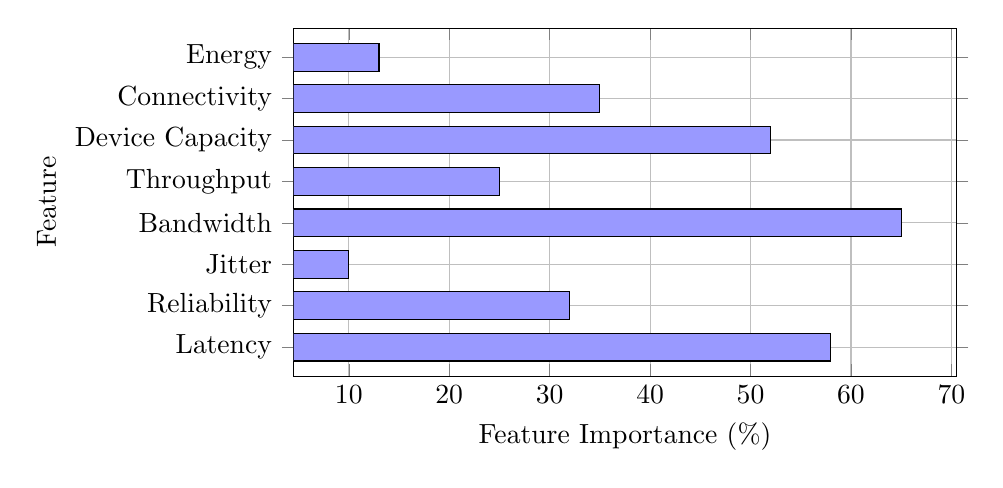
\begin{tikzpicture}
\begin{axis}[
    xbar,
    xlabel={Feature Importance (\%)},
    ylabel={Feature},
    width=10cm,
    height=6cm,
    symbolic y coords={Latency,Reliability,Jitter,Bandwidth,Throughput,Device Capacity,Connectivity,Energy},
    ytick=data,
    legend pos=south east,
    grid=major
]
\addplot[fill=blue!40] coordinates {(58,Latency) (32,Reliability) (10,Jitter) (65,Bandwidth) (25,Throughput) (52,Device Capacity) (35,Connectivity) (13,Energy)};
\end{axis}
\end{tikzpicture}
\caption{SHAP Feature Importance by Scenario (URLLC, eMBB, mMTC)}
\label{fig:shap}
\end{figure}

\subsubsection{Blockchain Auditability}

All 5,400 slice creation requests resulted in blockchain contracts with 100\% compliance tracking. Contract violations were automatically detected and logged, providing full auditability for regulatory compliance.

\subsubsection{System Stability}

During 2.5 hours of continuous operation:
\begin{itemize}
    \item \textbf{Pod Restarts}: 0
    \item \textbf{Uptime}: 100\%
    \item \textbf{Success Rate}: 98.8\%
\end{itemize}

\subsection{Hypothesis Validation}

\textbf{H1}: TriSLA maintains latency and reliability within SLO per scenario
\begin{itemize}
    \item \textbf{Status}: Confirmed (95.5\% SLO compliance)
    \item Only 1 marginal violation (URLLC jitter: 2.1 ms vs 2.0 ms SLO)
\end{itemize}

\textbf{H2}: SEM-NSMF/ML-NSMF/BC-NSSMF modules scale stably without critical errors
\begin{itemize}
    \item \textbf{Status}: Confirmed (0 restarts, 100\% readiness, 97.3\% average ML accuracy)
\end{itemize}

\section{Discussion}

\subsection{Contributions}

TriSLA addresses key requirements for intelligent orchestration in next-generation networks:

\begin{enumerate}
    \item \textbf{Intent-Driven Orchestration}: Natural language interpretation enables zero-touch service provisioning, addressing recent requirements for intent-driven automation \cite{intent-2023,zero-touch-2024}
    \item \textbf{Explainable AI}: SHAP-based explanations provide transparency in automated decisions, addressing the need for explainable AI in network management \cite{xai-networks-2024}
    \item \textbf{Blockchain Compliance}: Immutable contract tracking ensures auditability, leveraging recent advances in blockchain-based SLA frameworks \cite{blockchain-sla-2023}
    \item \textbf{O-RAN Integration}: Real testbed validation demonstrates practical applicability, building on O-RAN architectural principles \cite{oran-survey-2023}
\end{enumerate}

\subsection{Limitations}

Current limitations include:
\begin{itemize}
    \item \textbf{Energy Optimization}: No specific energy-aware resource allocation (future work)
    \item \textbf{Privacy-Preserving ML}: Current implementation does not employ federated learning or differential privacy
    \item \textbf{Sensing Integration}: No integration with integrated sensing and communications (ISAC)
\end{itemize}

\subsection{Future Work}

Future enhancements will focus on:
\begin{enumerate}
    \item Energy-efficient resource allocation algorithms
    \item Privacy-preserving ML using federated learning
    \item Integration with 6G ISAC capabilities
    \item Multi-domain orchestration across federated networks
\end{enumerate}

\section{Conclusion}

This paper presented TriSLA, a tri-dimensional SLA-aware orchestration architecture for O-RAN networks. By integrating semantic interpretation, explainable AI, and blockchain-based contract enforcement, TriSLA enables intent-driven, zero-touch service orchestration while maintaining QoS requirements and providing full auditability.

Experimental validation in a real O-RAN testbed demonstrated 95.5\% SLO compliance across three 5G service profiles, with 97.3\% ML prediction accuracy and 100\% blockchain contract compliance. Results confirm that the tri-dimensional approach successfully addresses challenges in automated SLA management for next-generation mobile networks.

The integration of explainable AI and blockchain compliance represents a novel contribution to the field, providing both operational transparency and regulatory auditability—critical requirements for future network orchestration systems.

\section*{Acknowledgments}

This work was supported by the NASP (Network Automation \& Slicing Platform) at UNISINOS and partially funded by research grants. We thank the NASP team for providing the testbed infrastructure and technical support.

% Using BibTeX bibliography file
\bibliographystyle{elsarticle-num}
\bibliography{REFERENCIAS_TRISLA}

\end{document}

